\textcolor{red}{AF: one thing is the problem and a different one is the solution, this section seems to talk about the solution, not the problem. A section about the problem should be added,}

\textcolor{red}{AF: a block diagram must be added and referred to.}

\begin{figure*}
	\centering
	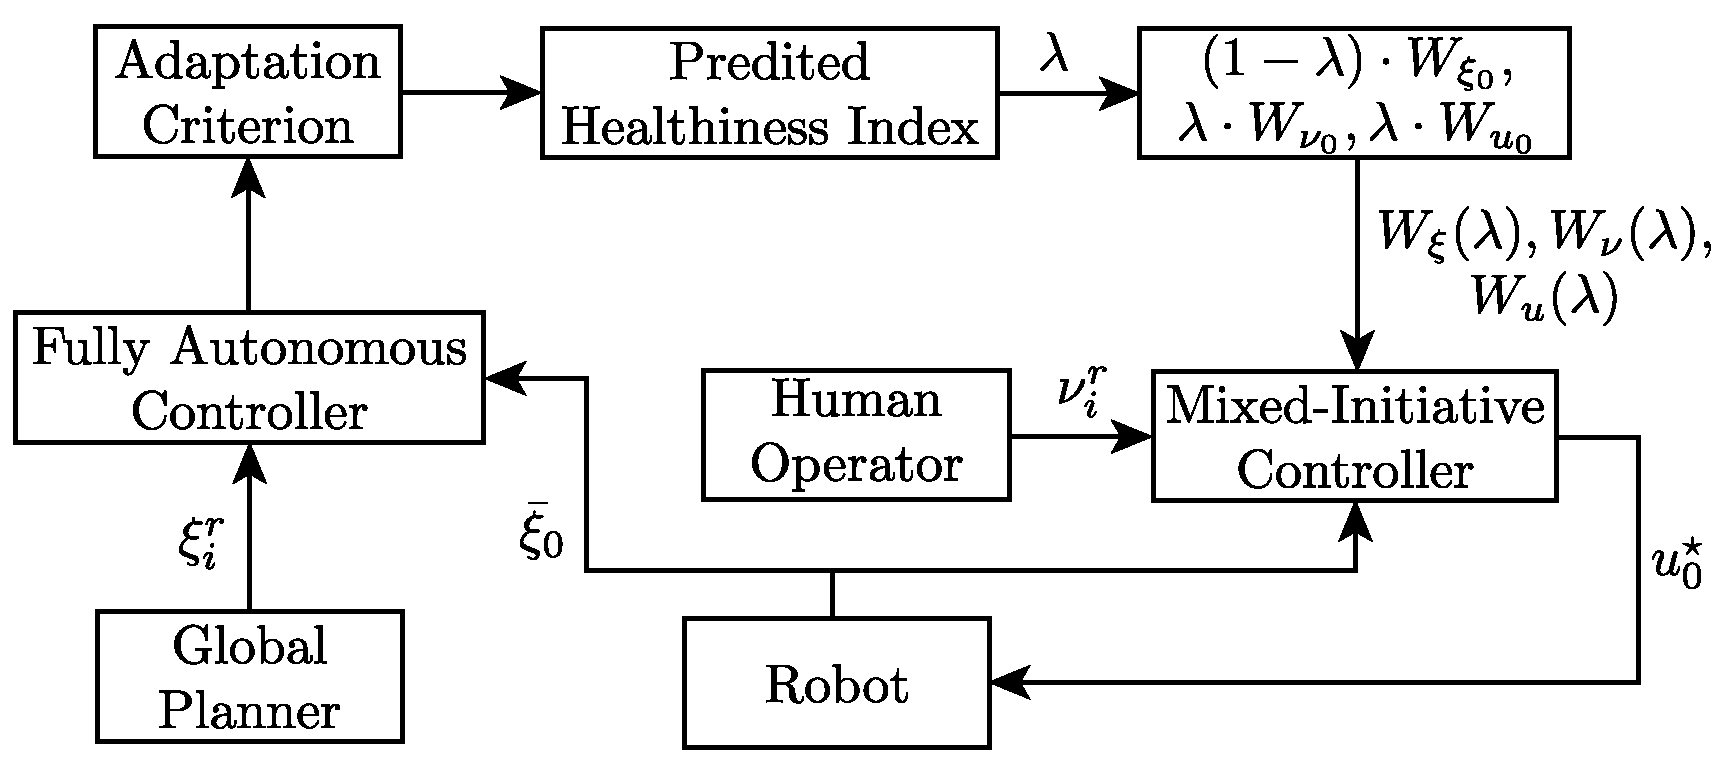
\includegraphics[width=1.0\textwidth]{figure/block_diagram}
\end{figure*}

The base controller of this work is a zone NMPC with trajectory-dependent penalty parameters. The zone NMPC model takes into account the robot dynamics plus part of the robot dynamics that the human is able to control, e.g. attitude and height \textcolor{red}{AF: to be checked}). The controller is driven by the predicted trajectories from another NMPC (namely, low-level NMPC), which considers just the dynamics of the robot. At each time instant, two constrained optimization problems are solved numerically, yielding two different feedback control policies.

In this section, we present the respective prediction models for each NMPC, as well as the nonlinear programs (NLP) arising in each NMPC formulation. 
%%%%%%%%%%%%%%%%%%%%%%%%%%%%%%%%%%%%%%%%%%%%%%%%%%%%%%%%%%%%%%%%%%%%%%%%%%%%%%%%%%%%%%
\subsection{Prediction Models}
Let $\{\mathcal{B}\}$ be the body-fixed frame, located at the center of mass (CoM) of a quadrotor, aligned with the North-West-Up (NWU) inertial frame $\{\mathcal{I}\}$. In order to implement the low-level NMPC, we consider a nonlinear dynamic model of the form
\begin{equation*}
	\dot{\xi} = f_1(\xi,u).
\end{equation*}
We then define the state vector, considering only the dynamics of the robot:
\begin{equation*}
	\xi := (p,\gamma,v_b,\omega,\Omega)^T \in \mathbb{R}^{16},
\end{equation*}
where $ p := (x, y, z)$  is the position vector in $\{\mathcal{I}\}$, $ \gamma := (\phi,\theta,\psi)$ are the Euler angles for orientation, $v_b := (v_x, v_y, v_z)$ is the linear velocities vector in $\{\mathcal{B}\}$, $\omega := (\omega_x, \omega_y, \omega_z)$ is the vector of angular rates, and finally $\Omega := (\Omega_1,\Omega_2,\Omega_3,\Omega_4)$ is the vector containing the rotation speed of the propellers. Hence, we regard the following quadrotor model:
 \begin{equation*}
 	\begin{aligned}
 	\dot{p} &= Rv_b \\
 	\dot{\gamma} &= T \omega\\
	\dot{v}_b &= \frac{1}{m}F - R^{T}G - \omega\times v_b\\
	\dot{\omega} &= J^{-1}(M - \omega\times J\omega)\\
	\dot{\Omega} &= \frac{\tau}{J_m},
 	\end{aligned}%
 \end{equation*}
 \textcolor{red}{AF: what about drag of the rotor in the motor equation?}
where the mass of the quadrotor is $m \in \mathbb{R}^+$, and $G \vcentcolon =(0, 0, mg)^T$ with $g$ being the gravitational acceleration. The robot inertia matrix with respect to its CoM and expressed in $\{\mathcal{B}\}$ is given by $J \vcentcolon = \text{diag}(J_{xx}, J_{yy}, J_{zz}) \in \mathbb{R}^{3 \times 3}$. The rotation matrix from  $\{\mathcal{B}\}$ to $\{\mathcal{I}\}$ is expressed as $R \in SO(3)$. The matrix $T \vcentcolon \mathbb{R}^3 \rightarrow \mathbb{R}^{3 \times 3}$ represents the relation between the instantaneous rates of change of the Euler angles and the instantaneous components of $\omega$. \textcolor{red}{AF: define ALL the symbols introduced, here and after} The total external forces and moments applied to the CoM of quadrotor in $\{\mathcal{B}\}$ are defined as 
 \begin{equation}
 	\begin{aligned}
    F & \vcentcolon =  \sum_{i=1}^4 C_T\Omega_{i}^2\mathbf{1}_z, \quad M \vcentcolon = (M_x, M_y, M_z)^T
	\end{aligned}
 \end{equation}\label{eq:force_moments}
 with
 \begin{equation*}
 	\begin{aligned}
    M_x &= C_T\cdot l(-\Omega_{1}^{2}-\Omega_{2}^{2}+\Omega_{3}^{2}+\Omega_{4}^{2}),\\
    M_y &= C_T\cdot l(-\Omega_{1}^{2}+\Omega_{2}^{2}+\Omega_{3}^{2}-\Omega_{4}^{2}),\\
    M_z &= C_D(-\Omega_{1}^{2}+\Omega_{2}^{2}-\Omega_{3}^{2}+\Omega_{4}^{2}),
 	\end{aligned}
 \end{equation*}
where $C_T$ is the thrust coefficient, $C_D$ is the drag coefficient, and $l$ is half of the distance between motors. When considering a medium-size quadrotor, the rotor inertia $J_m$ is not negligible as the radius of the rotor's axle is not small. Therefore, we consider the rotor torques as the control inputs of this system
\begin{equation}
	u := (\tau_1,\tau_2,\tau_3,\tau_4)^T \in \mathbb{R}^4.\label{eq:control_inputs}
\end{equation}



Moreover, for the zone NMPC let us consider the following nonlinear dynamic model:
\begin{equation*}
	\dot{\sigma} = f_2(\sigma,u).
\end{equation*}
This model is composed of the robot dynamics plus part of the robot dynamics that the human is able to control. For a quadrotor, the latter is essentially composed of the rotational dynamics and the translational dynamics in $z$ (which is directly linked to the collective speed of the propellers). Thus, we can formally define the part of the dynamics controlled by the human as:
\begin{equation*}
	\nu \vcentcolon = (\gamma, \omega, \Omega)^T \in \mathbb{R}^{10}.
\end{equation*}
Then, the state vector of the zone NMPC can be characterized as follows:
\begin{equation*}
	\sigma \vcentcolon = (p,\gamma,v_b,\omega,\Omega,\nu)^T \in \mathbb{R}^{26},
\end{equation*}
while the control inputs are the rotor torques, likewise regarded in \eqref{eq:control_inputs}.



\textcolor{red}{AF: this is confusing. Some of the states seem to appear twice. I would rather say that in this controller there are some additional exogenous inputs provided by the human which are the desired orientation and desired total thrust and give to these quantities a different name. In any case these quantities should not appear in the state of the robot, in the sense that they do not affect the robot dynamics directly, but rather in the objective function, i.e., in the controlled (closed loop) dynamics, in the same way the desired trajectory appear.}


%%%%%%%%%%%%%%%%%%%%%%%%%%%%%%%%%%%%%%%%%%%%%%%%%%%%%%%%%%%%%%%%%%%%%%%%%%%%%%%%%%%%%%
\subsection{Nonlinear Programs}
When using NMPC to control a system, at each sampling instant, a nonlinear nonconvex program is solved using the current state as the initial value. However, as the programs' solution times can be rather long, the employment of NMPC has only recently been extended to applications where shorter sampling times are required \cite{barros2020b}. Typically, a continuous-time, infinite-dimensional optimal control problem (OCP) is tailored according to the problem at hand, discretized using some numerical strategy, and then solved. In doing so, the tailored OCP is transformed into a discrete-time, finite-dimensional nonlinear program (NLP) for which the optimally conditions are set up and solved at each sampling instant. In our approach, we cast the mixed-initiative (MI) controller as a constrained NLP formulated as follows:

\begin{problem}[Mixed-Initiative Controller]
\begin{subequations}
{\!\!\!\!\!}{\!\!}\begin{align}
&\underset{\begin{subarray}{c}
\xi_0, \dots, \xi_N, \\
u_0, \dots, u_{N-1}
\end{subarray}}{\min}	    &&\sum_{i=0}^{N-1} L(\eta_i, \nu_i, \xi_i, u_i) + M(\eta_N, \nu_N,\xi_N)\\
&\,\,\,\quad \textnormal{s.t.}    &&\xi_0 - \Bar{\xi}_0 = 0, \label{eq:a}\\
& 						    &&\xi_{i+1} - F(\xi_i,u_i) = 0, \,\,\,\, i = 0,\dots, N-1,\\
& 						    &&\xi_i\in \mathcal{X}, \,\,\,\,\,\,\,\,\,\,\,\,\,\,\,\,\,\,\,\,\,\,\,\,\,\,\,\,\,\,\,\,\,\,\,\,\,\, i = 0,\dots, N-1,\label{eq:c}\\
& 						    &&u_i\in \mathcal{U},\label{eq:d} \,\,\,\,\,\,\,\,\,\,\,\,\,\,\,\,\,\,\,\,\,\,\,\,\,\,\,\,\,\,\,\,\,\,\,\,\,\, i = 0,\dots, N-1,
\end{align}{\!\!\!}
\end{subequations} where
\begin{equation*}
\begin{aligned}
		L(\eta_i, \nu_i, \xi_i, u_i) &\vcentcolon = \frac{1}{2}(\Delta\eta_i^T(1-\lambda)Q_{\eta}\Delta\eta_i + \Delta\nu_i^T\lambda Q_\nu\Delta\nu_i + \\
		& \,\,\,\,\,\,\,\,\,\,\,\,\,\,\,\,\,\Delta e_i^T(1-\lambda)Q_e\Delta e_i + u_i^T(1-\lambda)Ru_i)\\
		M(\eta_N, \nu_N,\xi_N) &\vcentcolon = \frac{1}{2}(\Delta\eta_N^T(1-\lambda)Q_{\eta_N}\Delta\eta_N + \\
		& \,\,\,\,\,\,\Delta\nu_N^T\lambda Q_{\nu_N}\Delta\nu_N + \Delta e_N^T(1-\lambda)Q_{e_N}\Delta e_N).
\end{aligned}
\end{equation*}\label{problem:mi}%
\end{problem}
Therein, stage and terminal cost terms are represented by $L$ and $M$, respectively. We denote the task variables tracking error as $\Delta\eta_i = \eta_i - \eta_i^r$, $\Delta\eta_N = \eta_N - \eta_N^r$, and the human inputs tracking error as $\Delta\nu_i = \nu_i - \nu_i^r$, $\Delta\nu_N = \nu_N - \nu_N^r$. The cost function also includes other penalty terms that might by relevant to the specific application. Their tracking errors are denoted as $\Delta e_i = h(\xi_i)-e_i^r$, and $\Delta e_N = h(\xi_N)-e_N^r$, where the output functions $h(\xi),\, h(\xi_N) \in \mathbb{R}^{n_h}$ and their respective references $e_i^r, e_N^r \in \mathbb{R}^{n_h}$ are defined by the relative complement $\mathbb{R}^{n_\xi} \setminus (\mathbb{R}^{n_\eta} \cup \mathbb{R}^{n_\nu})$. Note that $\xi \vcentcolon = (\xi_0, \dots, \xi_N)$ and $u \vcentcolon = (u_0,\dots,u_{N-1})$ represent the state and input trajectories of the discrete-time system whose dynamics are described by $F \vcentcolon \mathbb{R}^{n_{\xi}} \times \mathbb{R}^{n_u} \rightarrow \mathbb{R}^{n_{\xi}}$. 

Moreover, $\mathcal{X}$ and $\mathcal{U}$ implement the state and input constraints associated with the physical limitations of the robot. Denoted by $N$ is the horizon length and by $\bar{\xi}_0$ the current state estimate. The stage and terminal cost terms are weighted by the positive-definite weighting matrices $Q_{\eta}, Q_{\eta_N} \in \mathbb{R}^{n_\eta \times n_\eta}$, $Q_{\nu}, Q_{\nu_N} \in \mathbb{R}^{n_\nu \times n_\nu}$, $Q_{e}, Q_{e_N} \in \mathbb{R}^{n_h\times n_h}$, and $R \in \mathbb{R}^{n_u \times n_u}$. The scaling factor $\lambda \in (0,1)$ is the output of the blending mechanism and is used to determine how control authority should be mixed. Looking at the cost function, one can observe that increasing the value of $\lambda$ will give more weighting to keeping the human inputs closer than the motion generator commands. Note that we consider an open interval because we are interested in convex problems. Finally, once the solution is computed, the first element of the input trajectory $u_0$ is applied to the system before shifting the horizon forward in time (see Fig.~\ref{fig:block_diagram} for an illustration with the notations). 
%%%%%%%%%%%%%%%%%%%%%%%%%%%%%%%%%%%%%%%%%%%%%%%%%%%%%%%%%%%%%%%%%%%%%%%%%%%%%%%%%%%%%%